\chapter{Architecture}\label{ch:architecture}
API Scout is divided into three main parts: the backend, the databases, and the model.
A general architecture of the project can be found in Figure~\ref{fig:backend-architecture}.
In the backend, we have all those methods and APIs that deal with the embedding, indexing, and retrieval of the OpenAPI specifications.
For storing the data, we use both a MongoDB and an Elasticsearch instance.
The MongoDB instance is used for storing the OpenAPI json files.
On the other hand, the Elasticsearch instance is used to store the metadata -- used by the DSL -- and the vector embeddings of the specifications. \\ \\
From a tech stack point of view, we can see in Figure~\ref{fig:languages-architecture} that we used both Elasticsearch and MongoDB for the databases, Tensorflow for the embedding model, and Golang for the backend.

\begin{figure}[h]
    \begin{center}
        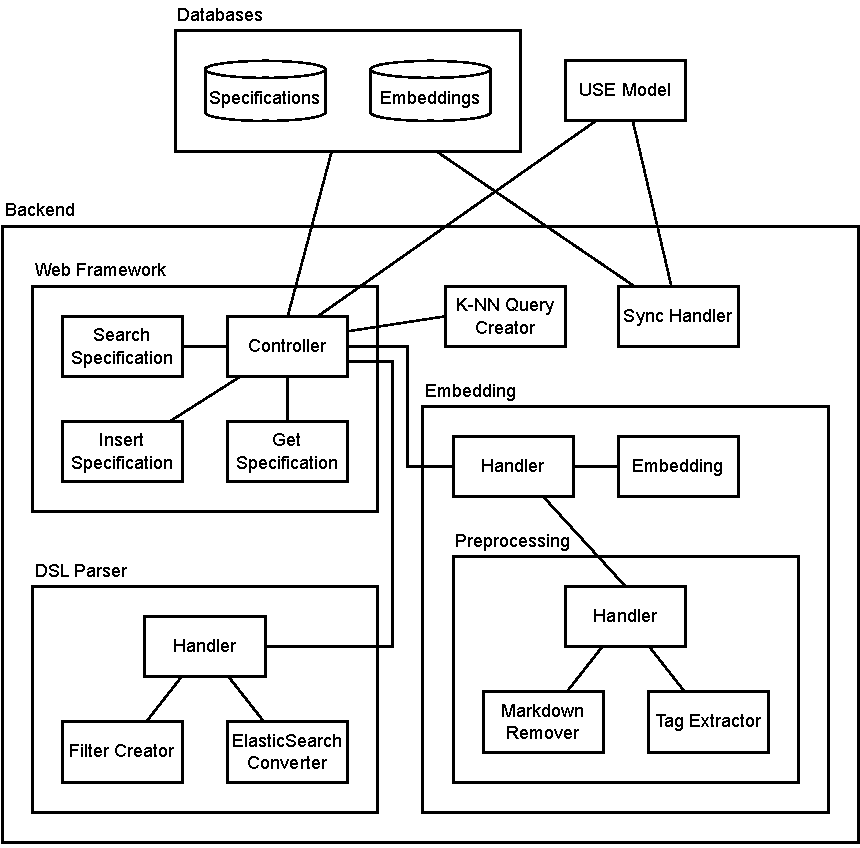
\includegraphics[width=0.6\linewidth]{assets/pdf/architecture/general-architecture}
    \end{center}

    \caption{API Scout's architecture}
    \label{fig:backend-architecture}
\end{figure}

\begin{figure}[h]
    \begin{center}
        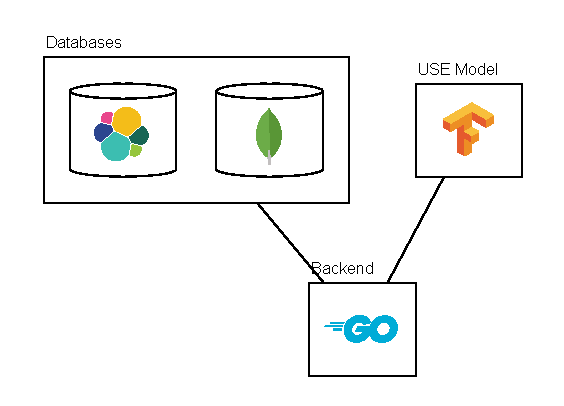
\includegraphics[width=0.6\linewidth]{assets/pdf/architecture/languages-architecture}
    \end{center}

    \caption{API Scout's tech stack}
    \label{fig:languages-architecture}
\end{figure}

\section{Databases}\label{sec:databases}

The system uses two databases to store the data, a MongoDB and an Elasticsearch database.
In the following sections, we will explain more in depth the reasons behind choosing two different databases and how they are used.

\subsection{Specifications Database}\label{subsec:specifications-database}
The specifications database is a MongoDB instance.
Since OpenAPI has multiple versions, and not all API specifications adhere to this standard, it is possible that the specifications have a slightly different structure.
The reason behind choosing only some of the fields of the original dataset is that we consider these to be the most relevant when building a retrieval system and a filtering DSL\@.
We used MongoDB to save the OpenAPI specifications both because MongoDB handles well these kind of JSON/YAML documents, and because other API Analytics services -- outside the scope of this thesis, but which provide the source of the dataset -- rely on such database and data structure~\cite{souhaila_serbout_apistic_2024}. \\ \\
The MongoDB database is composed of two collections, one containing the specifications and one containing the metrics for those specifications.

\subsubsection{Specifications Collection}
In the specifications collection, we have all the specifications that have been scraped from different sources: GitHub, BigQuery, APIs.guru and SwaggerHub~\cite{souhaila_serbout_apistic_2024}.
Moreover, the documents have been saved with two different structures.
The structure of the documents coming from SwaggerHub is described in Listing~\ref{lst:data-swaggerhub} and Table~\ref{tab:data-swaggerhub}.
The structure of the documents coming from GitHub, instead, is described in Listing~\ref{lst:data-github} and Table~\ref{tab:data-github}.
In Tables~\ref{tab:data-swaggerhub} and~\ref{tab:data-github}, we describe what each top-level field in the document means.
In addition, we also highlight those fields that have been used in API Scout.

\begin{lstlisting}[label={lst:data-swaggerhub},language=json,caption={Structure of the data coming from SwaggerHub},captionpos=b]
          {
              "_id": ObjectId("65ce1ae96eb5a9c18ffe38fc"),
              "_fetching_reference": null,
              "_API_reference": "https://api.swaggerhub.com/...",
              "_meta": {},
              "_name": "Bisan Enterprise API",
              "_description": "This is the Bisan...",
              "_created_at": "2020-12-15T09:42:49Z",
              "_last_modified": "2020-12-15T09:42:49Z",
              "_created_by": "mbanna",
              "_API_url": "https://api.swaggerhub.com/.../1.0.1",
              "_version": "1.0.1",
              "_OPENAPI_version": "3.0.0",
              "_API_spec_hash": null,
              "_API_url_hash": "7b88c0cjh4a34vdb78...",
              "api": {}
          }
\end{lstlisting}

\begin{lstlisting}[label={lst:data-github},language=json,caption={Structure of the data coming from GitHub},captionpos=b]
           {
               "_id": ObjectId("65ce1ae96eb5a9c18ffe38fc"),
               "id": 187463,
               "api_spec_id": 472773,
               "api_title": "math-api-v1",
               "api_version": "1.0",
               "commit_date": 2019-11-27T12:31:23.000+00:00,
               "commits": 1,
               "processed_at": 2023-11-27T12:31:23.000+00:00,
               "sha": "vsd876vs68df68fs...",
               "url": "https://raw.githubusercontent.com/...",
               "latest": true,
               "api": {}
           }
\end{lstlisting}

\subsubsection{Metrics Collection}
In the metrics collection, we have one document for each specification.
The connection between the documents is done through the MongoID. If the MongoID in the specification collection and the one in the metrics collection are the same, this means that the two documents are related.
The metrics documents store some statistics about the corresponding OpenAPI specification.
Listing~\ref{lst:data-metrics} and Table~\ref{tab:data-metrics} describe the structure of these documents.
Moreover, as before, we also highlight those fields that have been used in API Scout.

\begin{lstlisting}[label={lst:data-metrics},language=json,caption={Structure of the specification's metrics data},captionpos=b]
            {
                "_id": ObjectId("65ce1ae96eb5a9c18ffe38fc"),
                "securityData": {
                    "schemes": [],
                    "endpointsCount": 20,
                    "average": 10
                },
                "schemas": [],
                "schemaSize": {
                    "schemas": 3,
                    "defined_schemas": 3,
                    "properties": 5,
                    "max_properties": 2,
                    "min_properties": 1
                },
                "structureSize": {
                    "paths": 3,
                    "operations": 3,
                    "used_methods": 3,
                    "used_parameters": 2
                },
                "documentationsData": {}
            }
\end{lstlisting}

\begin{table}[!h]
    \begin{center}
        \begin{tabular}{l p{11cm} c}
            \hline
            \textbf{Field} & \textbf{Description} & \textbf{Used} \\ \hline
            \verb|_id| & The ID given to the document by MongoDB & \cmark \\
            \verb|_fetching_reference| & The ID given by the crawler to the document & \xmark \\
            \verb|_API_reference| & The URL of the API & \xmark \\
            \verb|_meta| & Some metadata on the API server and validity of the JSON specification & \xmark \\
            \verb|_name| & The name of the API (taken from the API specification) & \cmark \\
            \verb|_description| & The description of the API (taken from the API specification) & \xmark \\
            \verb|_created_at| & The date of creation of the API & \cmark \\
            \verb|_last_modified| & The date the API was last modified & \xmark \\
            \verb|_created_by| & The user that uploaded the API specification & \xmark \\
            \verb|_API_url| & The specific URL for the specification version & \xmark \\
            \verb|_version| & The API version & \cmark \\
            \verb|_OPENAPI_version| & The OpenAPI version used in the specification & \cmark \\
            \verb|_API_spec_hash| & The specification hash & \xmark \\
            \verb|_API_url_hash| & The URL hash & \xmark \\
            \verb|api| & The object containing the API specification & \cmark \\ \hline
        \end{tabular}
    \end{center}

    \caption{Description of the data contained in a SwaggerHub document}
    \label{tab:data-swaggerhub}
\end{table}

\begin{table}[!h]
    \begin{center}
        \begin{tabular}{l l c}
            \hline
            \textbf{Field} & \textbf{Description} & \textbf{Used} \\ \hline
            \verb|_id| & The ID given to the document by MongoDB & \cmark \\
            \verb|id| & The ID of the API specification's commit & \xmark \\
            \verb|api_spec_id| & The ID of the API specification & \cmark \\
            \verb|api_title| & The name of the API & \cmark \\
            \verb|api_version| & The version of the API & \cmark \\
            \verb|commit_date| & The time at which this version was committed & \cmark \\
            \verb|commits| & The number of commits this API has in total & \cmark \\
            \verb|processed_at| & The time at which the API was processed by the crawler & \xmark \\
            \verb|sha| & The hash of the specification & \xmark \\
            \verb|url| & The URL of the specification & \xmark \\
            \verb|latest| & If the current commit is the latest or not & \cmark \\
            \verb|api| & The object containing the API specification & \cmark \\ \hline
        \end{tabular}
    \end{center}

    \caption{Description of the data contained in a GitHub document}
    \label{tab:data-github}
\end{table}

\begin{table}[!h]
    \begin{center}
        \begin{tabular}{l p{9.5cm} c}
            \hline
            \textbf{Field} & \textbf{Description} & \textbf{Used} \\ \hline
            \verb|_id| & The ID given to the document by MongoDB & \cmark \\
            \verb|securityData.schemes| & A list of all the security schemes present in the specification & \xmark \\
            \verb|securityData.endpointsCount| & The number of endpoints covered by some kind of security schema & \cmark \\
            \verb|securityData.average| & The average number of endpoints covered by some kind of security schema & \xmark \\
            \verb|schemas| & A list of all the schemas present in the specification & \xmark \\
            \verb|schemaSize.schemas| & The number of schemas used in the specification & \cmark \\
            \verb|schemaSize.defined_schemas| & The number of defined schemas in the specification & \xmark \\
            \verb|schemaSize.properties| & The number of properties used in the specification & \cmark \\
            \verb|schemaSize.max_properties| & The maximum number of properties used in a schema & \xmark \\
            \verb|schemaSize.min_properties| & The minimum number of properties used in a schema & \xmark \\
            \verb|structureSize.paths| & The number of paths in the specification & \cmark \\
            \verb|structureSize.operations| & The number of operations in the specification & \cmark \\
            \verb|structureSize.used_methods| & The number of methods used in the specification & \cmark \\
            \verb|structureSize.used_parameters| & The number of parameters used in the specification & \xmark \\
            \verb|documentationsData| & Object containing metrics about the documentation of endpoints & \xmark \\ \hline
        \end{tabular}
    \end{center}

    \caption{Description of the data contained in a metrics document}
    \label{tab:data-metrics}
\end{table}

\subsection{Embeddings Database}\label{subsec:embeddings-database}
To search for API specifications by querying their natural language descriptions, however, we need to save the vectorization of the natural language extracted from the OpenAPI Specification somewhere.
Since the MongoDB data structure could not be modified, the chosen database for storing the vectors was Elasticsearch -- which also contains metadata and metrics of the API specifications. \\ \\
The reason behind choosing Elasticsearch is that it offers out-of-the-box solutions to deal with textual embeddings.
For instance, the embeddings -- when indexed -- are saved into a Hierarchical Navigable Small World graph (Section ~\ref{subsec:hierarchical-navigable-small-world-graphs}), which helps with retrieval performance.
In addition, it already offers an approximate K-NN search (Section~\ref{subsec:hierarchical-navigable-small-world-graphs}) API with the possibility of pre- or post-filtering the data.
The aforementioned metadata and metrics are used to pre-filter the data in the K-NN search queries.

\section{Universal Sentence Encoder Model}\label{sec:use-model}

To create the vector embeddings of the OpenAPI specifications, we rely on an external Docker container.
This Docker container is based on the \verb|tensorflow/serving| image, which enables us to perform REST API calls to the deep learning model we use for the embedding.
The model chosen for this project is the Universal Sentence Encoder (USE) by Google (Section~\ref{subsec:document-embedding}). \\ \\
The model, after being sent some text fragments as input, will return one 512-dimension vector embedding for each fragment sent to the model.
In practice, the Docker compose requires the request to be structured as in Listing~\ref{lst:model-request}, and the response to be structured as in Listing~\ref{lst:model-response}.

\begin{center}
    \begin{lstlisting}[label={lst:model-request},language=json,caption={Example of request body sent to the model},captionpos=b]
                       {
                           "instances": [
                               "a random fragment",
                               ...
                           ]
                       }
    \end{lstlisting}
\end{center}

\begin{center}
    \begin{lstlisting}[label={lst:model-response},language=json,caption={Example of response body sent to the model},captionpos=b]
                           {
                               "predictions": [
                                   [
                                       0.12321,
                                       0.23123,
                                       ...
                                   ],
                                   ...
                               ]
                           }
    \end{lstlisting}
\end{center}

\section{Web Framework}\label{sec:web-framework-1}
The Web framework module handles all the connections made by external users to the service.
The framework publishes several different endpoints, as well as a Swagger documentation page of the exposed endpoints. \\ \\
The endpoints handle the basic operations of the tool, namely indexing, searching, and retrieving.
Moreover, there are two more endpoints that are used as helpers for migration of the data and evaluation of the system's performance.

\subsection{Indexing Endpoint}\label{subsec:indexing-endpoint-1}
The indexing endpoint (\verb|POST| \verb|/api/v1/specification|) is used to insert new OpenAPI specifications in both MongoDB and Elasticsearch (Figure~\ref{fig:flow-index}). \\ \\
The endpoint takes an OpenAPI specification wrapped in an \verb|api| object, it extracts the natural language fields from it, and then passes it to the main pipeline.
The pipeline is composed of an embedding pipeline component -- which creates the vector embeddings for the specification, and an indexing component.
The latter is used to structure the specification in the correct way and send it both to MongoDB and to Elasticsearch.
To MongoDB, it will send the entire specification, while to Elasticsearch it will send the metadata -- if present -- together with the vector embedding of the document.

\begin{figure}[!h]
    \begin{center}
        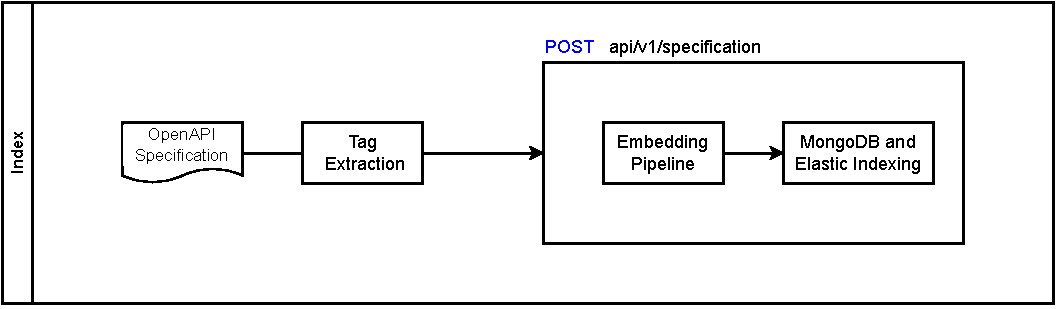
\includegraphics[width=0.8\linewidth]{assets/pdf/architecture/flow-index}
    \end{center}

    \caption{Conceptual view of the indexing pipeline}
    \label{fig:flow-index}
\end{figure}

\subsection{Search Endpoint}\label{subsec:search-endpoint-1}
In the case of the search endpoint (\verb|POST| \verb|/api/v1/search|), the user will be able to send either a specification fragment or a query, some filters, and parameters relative to the pagination and the K-NN query (Figure~\ref{fig:flow-search}).
The reason we chose a \verb|POST| request instead of a \verb|GET| request, is that the query plus the filters would have resulted in a URL that could be too long for the browser or tool to handle, thus we opted for a \verb|POST| request with a body. \\ \\
After passing a query or a specification to the endpoint, it will be preprocessed and fed to the main pipeline.
This pipeline consists of two main components, the embedding pipeline component and the DSL parsing component.
While the former creates the vector embedding from the preprocessed specification, the latter will extract the DSL field of the request and translate our DSL language into API calls that Elasticsearch uses to make its API calls.
Finally, the search query is sent to Elasticsearch, which will retrieve the most similar documents to the query.
Moreover, several calls will be made to MongoDB to retrieve the json specifications -- if requested by the user.

\begin{figure}[!h]
    \begin{center}
        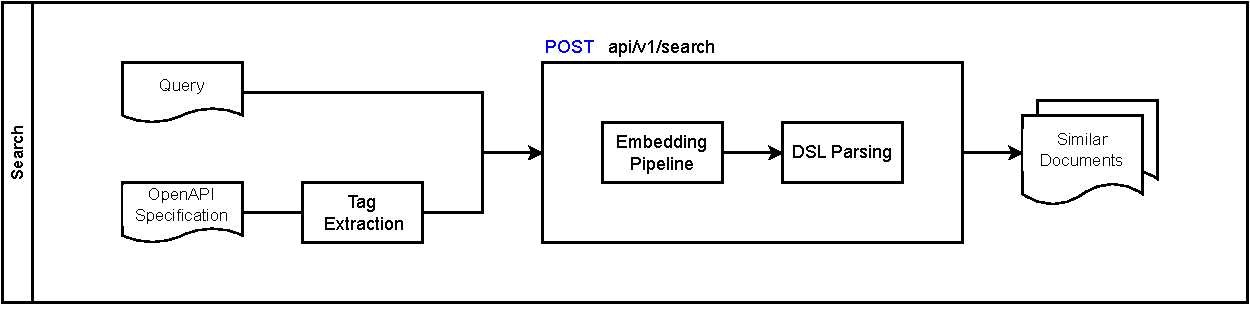
\includegraphics[width=0.9\linewidth]{assets/pdf/architecture/flow-search}
    \end{center}

    \caption{Conceptual view of the search pipeline}
    \label{fig:flow-search}
\end{figure}

\subsection{Retrieval Endpoint}\label{subsec:retrieval-endpoint-1}
The retrieval endpoint (\verb|GET| \verb|/api/v1/specification/{id}|) is used to get a specific OpenApi specification (Figure~\ref{fig:flow-retrieve}).
This endpoint will simply search for the given id in both the Elasticsearch and MongoDB databases, and return a document which will be a combination of the two documents returned by the two databases.

\begin{figure}[!h]
    \begin{center}
        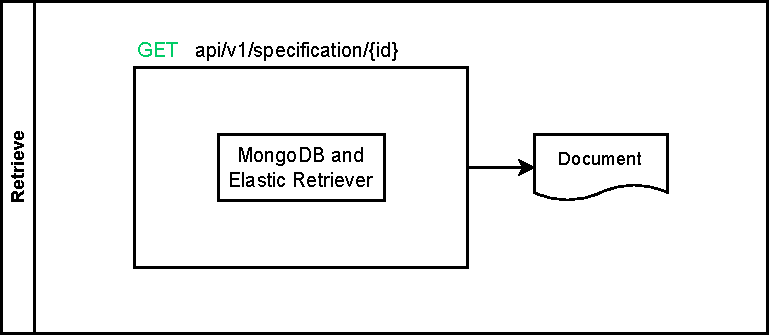
\includegraphics[width=0.5\linewidth]{assets/pdf/architecture/flow-retrieve}
    \end{center}

    \caption{Conceptual view of the retrieval pipeline}
    \label{fig:flow-retrieve}
\end{figure}

\subsection{Preprocessing Endpoint}\label{subsec:preprocessing-endpoint-1}
The preprocessing endpoint (\verb|POST| \verb|/api/v1/preprocess|) is used to simulate the preprocessing step for a search query (Figure~\ref{fig:flow-preprocess}).
This endpoint has been implemented has a helper endpoint during the evaluation process of this thesis. \\ \\
A document or query is passed as input to the endpoint.
The document will then go through a preprocessing pipeline.
In this pipeline, all the natural language tags will be extracted from the document, and then the resulting string will be cleaned of every markdown structure.
The endpoint will then return to the user a string representing the cleaned version of the input.
In a normal scenario -- i.e.\ in the case of a search or indexing query -- this string will be passed to the embedding model which will use the text to create a vector embedding for the OpenAPI specification or the query.

\begin{figure}[!h]
    \begin{center}
        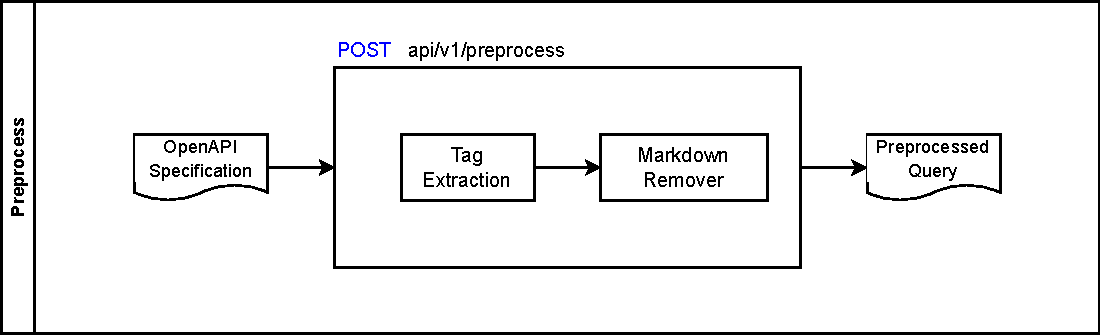
\includegraphics[width=0.8\linewidth]{assets/pdf/architecture/flow-preprocess}
    \end{center}

    \caption{Conceptual view of the preprocessing pipeline}
    \label{fig:flow-preprocess}
\end{figure}

\subsection{Synchronization Endpoint}\label{subsec:synchronization-endpoint-1}
The synchronization endpoint (\verb|PUT| \verb|/api/v1/sync|) is an idempotent endpoint used to index documents that are present in the MongoDB database in Elasticsearch (Figure~\ref{fig:flow-sync}). \\ \\
This endpoint will make sure that the two databases are always in sync.
If, while going through the MongoDB documents, it finds a document that is already in the Elasticsearch database, then it will not insert it again -- from here the idempotence and the choosing of the \verb|PUT| method for this endpoint.

\begin{figure}[!h]
    \begin{center}
        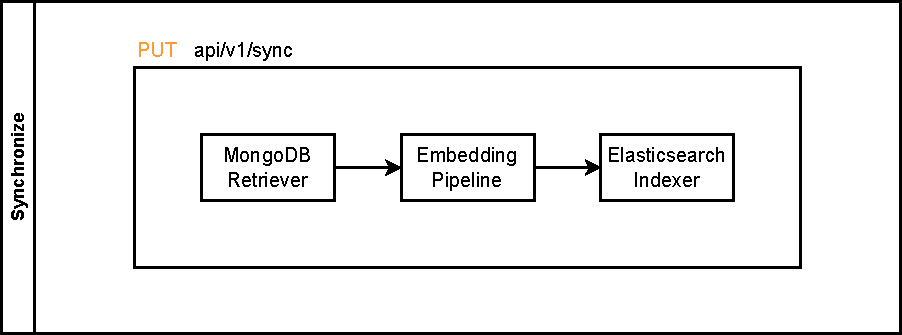
\includegraphics[width=0.7\linewidth]{assets/pdf/architecture/flow-sync}
    \end{center}

    \caption{Conceptual view of the synchronization pipeline}
    \label{fig:flow-sync}
\end{figure}

\section{Preprocessing and Embedding}\label{sec:preprocessing-and-embedding}
Preprocessing and embedding of queries are done inside the \verb|embedding| group of components.
In this group, the system receives the embedding from the web framework controller, and starts the embedding process.
Before transforming the specification into a vector of floating point numbers, it must be preprocessed. \\ \\
In the preprocessing stage, we extract all the specification tags that contain natural language.
After the extraction of these values, they are all inserted into a string which is passed to the Markdown remover component.
This component will strip from the string all of those symbols and structures that are used to defined Markdown components.
Moreover, the string is cleaned of all URL, even if they are not in a Markdown format. \\ \\
Once the string has been properly cleaned, it is passed to the USE model via a POST request.
The model will then return a 512-dimension array of floating point numbers representing the string in a 512-dimensional space.

